\documentclass[12pt]{article} 
\usepackage[utf8]{inputenc}
\usepackage[T2A]{fontenc}
\usepackage{amsthm}
\usepackage{amssymb}
\usepackage{blindtext}
\usepackage{amsmath}
\usepackage{tikz} 
\usepackage{listings}
\usepackage{xcolor}
\usepackage{float}
\usepackage{graphicx}
\usepackage{hyperref}
\usepackage{wrapfig}
\hypersetup{
    colorlinks=true,
    linkcolor=blue,
    filecolor=blue,      
    urlcolor=blue,
    pdftitle={Overleaf Example},
    pdfpagemode=FullScreen,
    }
\graphicspath{ {./images} }

\title{Bioinformatics HW4}
\author{Ershov Ivan}
\date{December 2021}

\begin{document}
\maketitle
Я выбрал из базы человека с \href{https://opensnp.org/users/10161}{ID=8427}\\\\
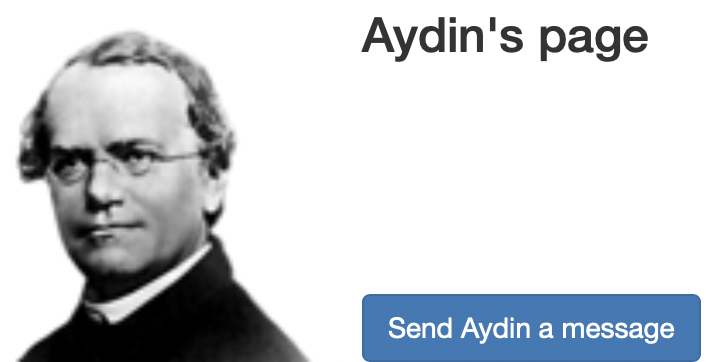
\includegraphics[width=\textwidth]{images/person.png}\\\\
\newpage
\paragraph{Задание 1. Какой наиболее вероятный цвет глаз у этого человека?
\\}
Для обределения цвета глаз у человека (согласно ресурсу \href{https://hirisplex.erasmusmc.nl}{IrisPlex}) нам нужны слудющие SNP: rs12913832, rs1800407, rs12896399, rs16891982, rs1393350, rs12203592. Найдем их в скаченном файле:\\\\
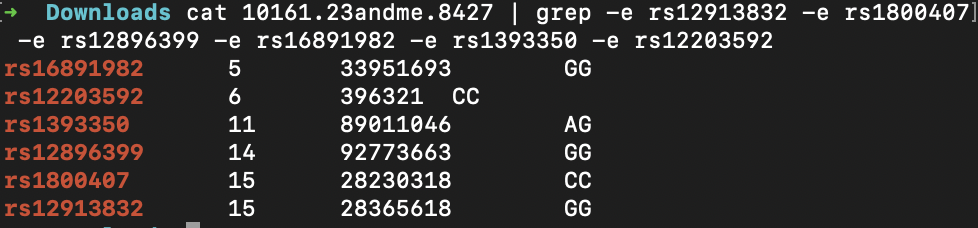
\includegraphics[width=\textwidth]{images/image0.png}\\\\
Теперь воспользуемся принципом комплементарности и внесем найденные генотипы:\\\\
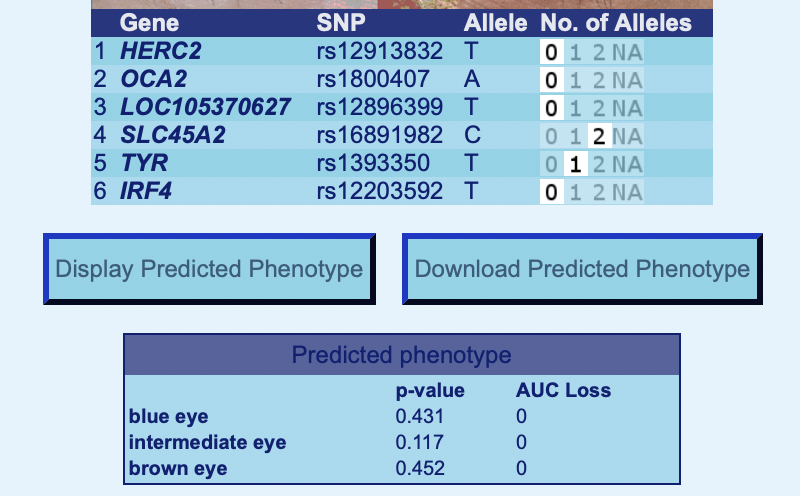
\includegraphics[width=\textwidth]{images/image1.png}\\\\
\textbf{В итоге получаем,} что у выбранного мной человека вероятнее всего коричневый цвет глаз (brown eye имеет наибольшее p-value)
\newline

\paragraph{Задание 2. Повышен или понижен риск тромбоза у данного человека?
\\}
Найдем нужные нам SNP в файле:\\\\
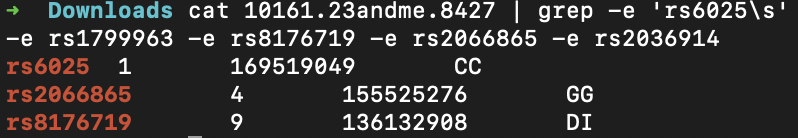
\includegraphics[width=\textwidth]{images/image2.png}\\\\
Найдено только 3 SNP, один из которых с пометкой DI. Этого не будет достаточно для точного вывода о предрасположенности. Исследовать будем только rs6025 и rs2066865. Найдем их в SNPedia:\\\\
rs6025:\\
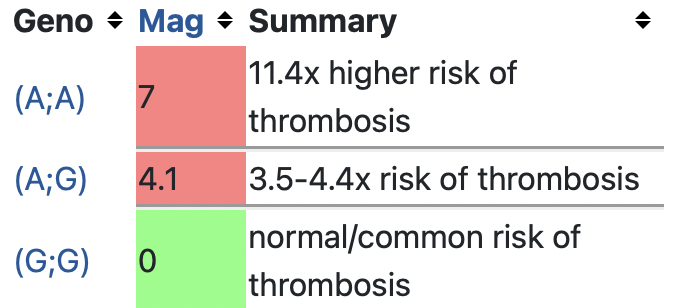
\includegraphics[width=\textwidth]{images/rs6025.png}\\\\
rs2066865:\\
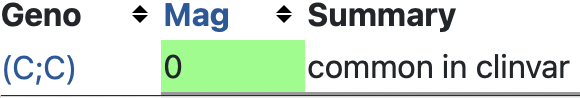
\includegraphics[width=\textwidth]{images/rs2066865.png}\\\\
(G,G) комплементарно (C, C), поэтому по SNP rs6025 сделаем вывод, что рискованного генотипа у выбранного человека нет, поэтому можно считать, что риск тромбоза в пределах нормы. 
\newpage
\paragraph{Задание 3-5. Из snpedia выбрать три разных интересных снипа и проверить на предрасположенность/связи с тем или иным признаком\\}
Выберем следующие три снипа:

Найдем выбранные SNP:\\\\
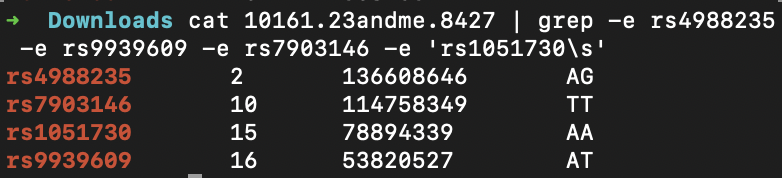
\includegraphics[width=\textwidth]{images/image3.png}\\\\
Исседуем и сделаем выводы:
\newpage

\textbf{1)} \href{https://www.snpedia.com/index.php/Rs4988235}{rs4988235} неперносимость лактозы\\\\

\includegraphics[width=\textwidth]{images/image4.png}\\
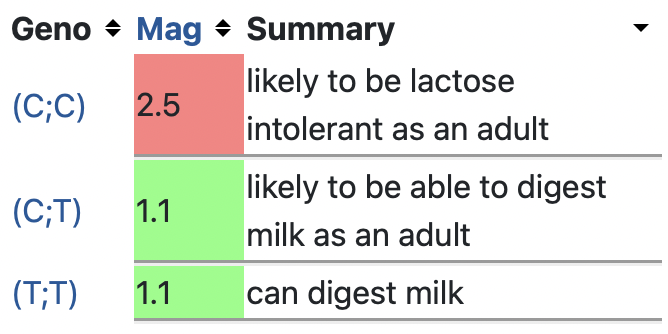
\includegraphics[width=\textwidth]{images/rs4988235.png}\\\\
Заметим, что на данной позиции генотип человека AG, что по комплементарности даст TC=CT, поэтому можем сделать вывод, что есть \textbf{очень маленькая} вероятность того, что у человека может быть непереносимость лактозы.
\newpage

\textbf{2)} \href{https://www.snpedia.com/index.php/Rs9939609}{rs9939609} риск ожирения и развития диабета 2-го типа\\\\

\includegraphics[width=\textwidth]{images/image5.png}\\
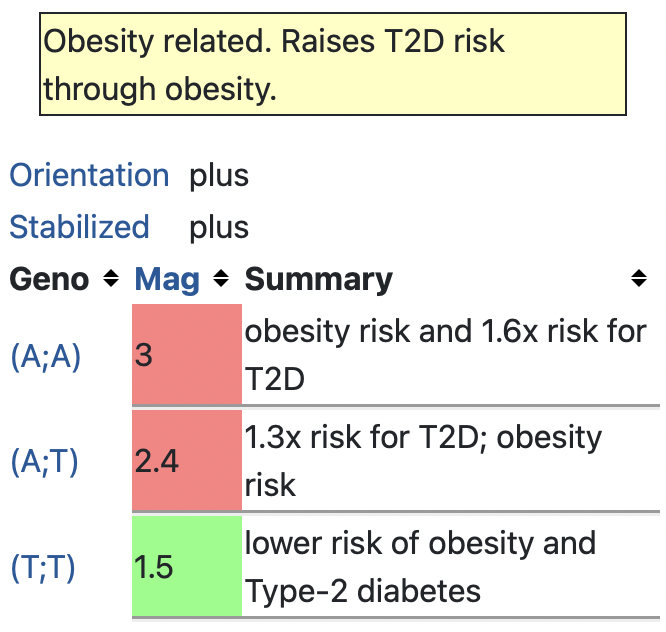
\includegraphics[width=\textwidth]{images/rs9939609.png}\\\\
Заметим, что на данной позиции генотип человека AT, поэтому можем сделать вывод, что есть у выбранного человека повышенный риск ожирения и диабета 2-го типа.
\newpage

\textbf{3)} \href{https://www.snpedia.com/index.php/Rs7903146}{rs7903146} риск развития диабета 2-го типа\\\\

\includegraphics[width=\textwidth]{images/image6.png}\\
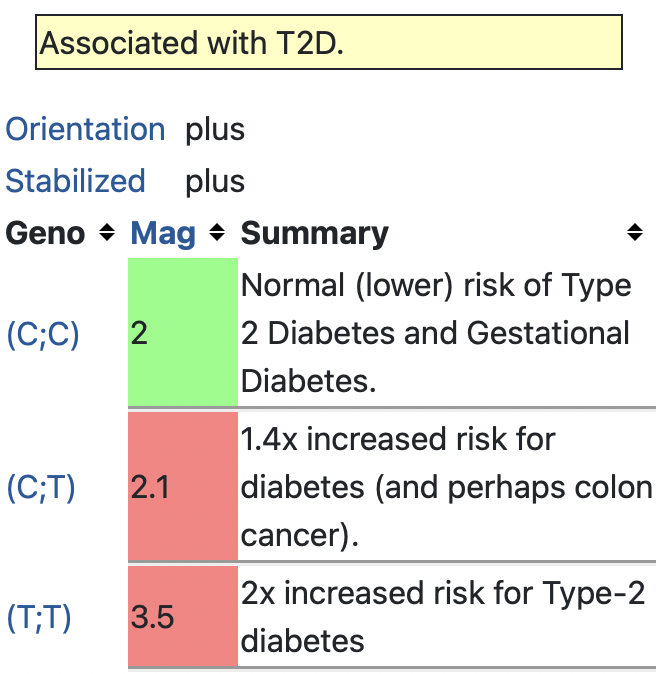
\includegraphics[width=\textwidth]{images/rs7903146.png}\\\\
Заметим, что на данной позиции генотип человека TT, поэтому можем сделать вывод, что есть у выбранного человека значительно повышенный риск развития диабета 2-го типа.
\newpage

\textbf{4)} \href{https://www.snpedia.com/index.php/Rs1051730}{rs1051730} повышенный риск заболеваний, вызываемые алкоголем или курением\\\\

\includegraphics[width=\textwidth]{images/image7.png}\\\\
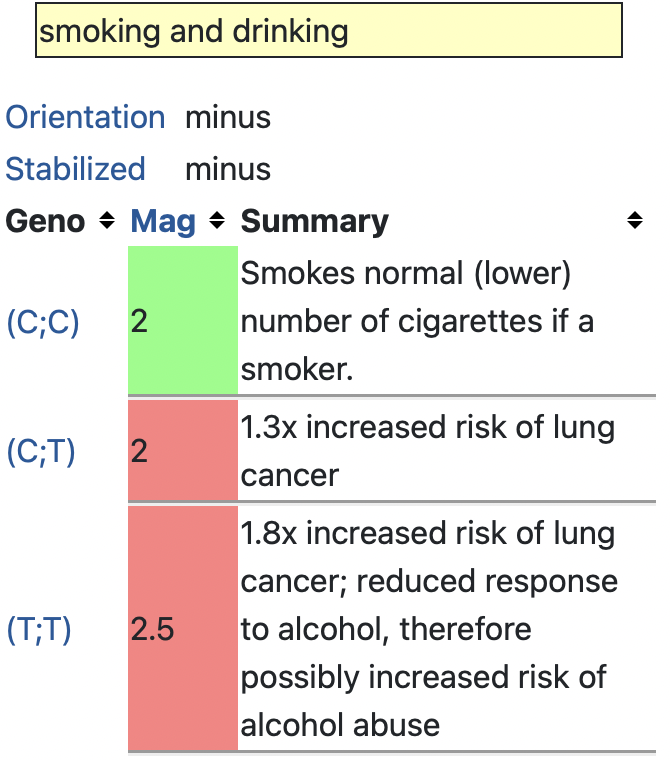
\includegraphics[scale=1.03]{images/rs1051730.png}\\\\
Заметим, что на данной позиции генотип человека AA, что по комплементарности даст TT, поэтому можем сделать вывод, что у человека есть повышенный риск рака легких, также можно заметить, что у человека понижена реакция на алкоголь, что может привести к злоупотреблению алкоголем.
\end{document}